%!TEX root = ../../../main.tex

	% \section{Photostability} \label{subsec::photostab}
	%
	%
	% \begin{figure}[tp]
	% 	\begin{subfigure}[tp]{ 0.49\linewidth}
	% 		\caption{}\label{subfig::blink_long}
	% 		\centering
	% 		\testbox{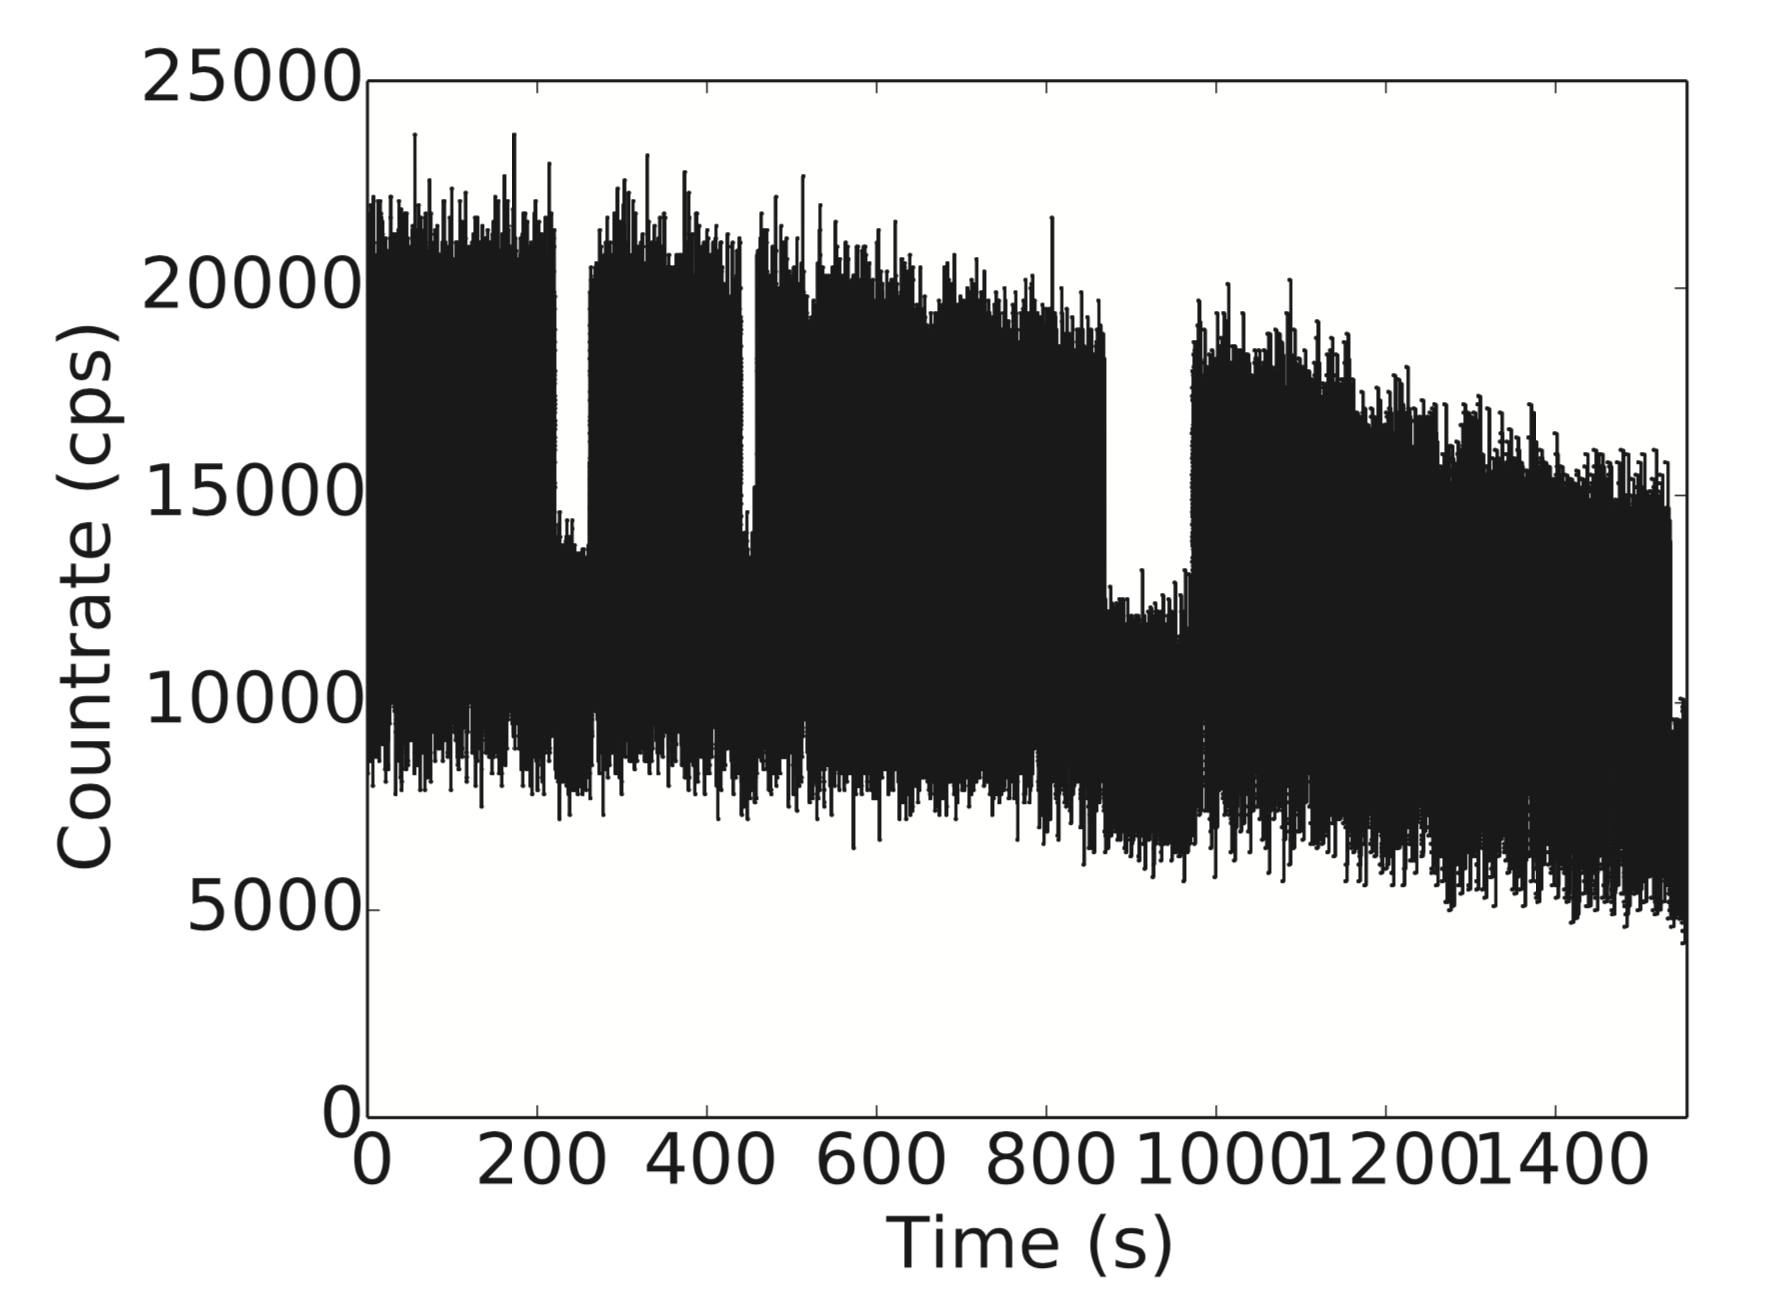
\includegraphics[trim = 0 0 0 0,  clip= true, width = \textwidth]{./pics/Ir8_g2zuSpektrum8_15_5_countrate_0_01_conv_screenshot.png}}
	% 	\end{subfigure}
	% 	\hfill
	% 	\begin{subfigure}[tp]{ 0.49\linewidth}
	% 		\caption{}\label{subfig::blink_short}
	% 		\centering
	% 		\testbox{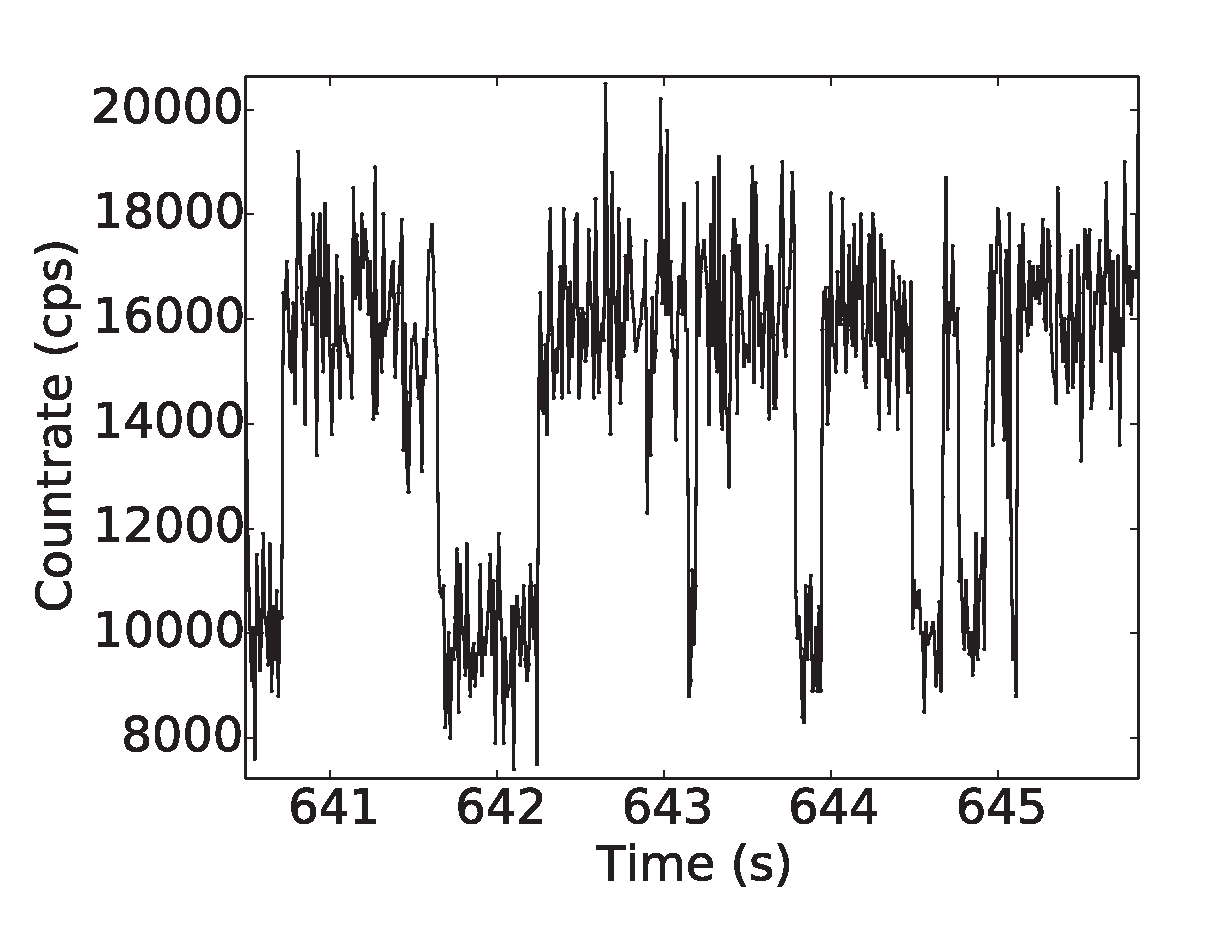
\includegraphics[trim = 0 0 0 0,  clip= true, width =\textwidth]{./pics/Ir8_g2zuSpektrum8_15_5_countrate_0_01_conv_detail.pdf}}
	% 	\end{subfigure}
	% 	\caption{Distribution of countrate of a blinking level vs. its retention time in this level. (a) Time trace of the single emitter exhibiting the highest blinking rate. The variation of the countrate in the upper state is attributed to a drift of the setup. (b) Detail of the time trace of the same emitter.}
	% 	\label{fig::blink}
	% \end{figure}
	%
	% \begin{figure}[tp]
	% 	\centering
	% 	\testbox{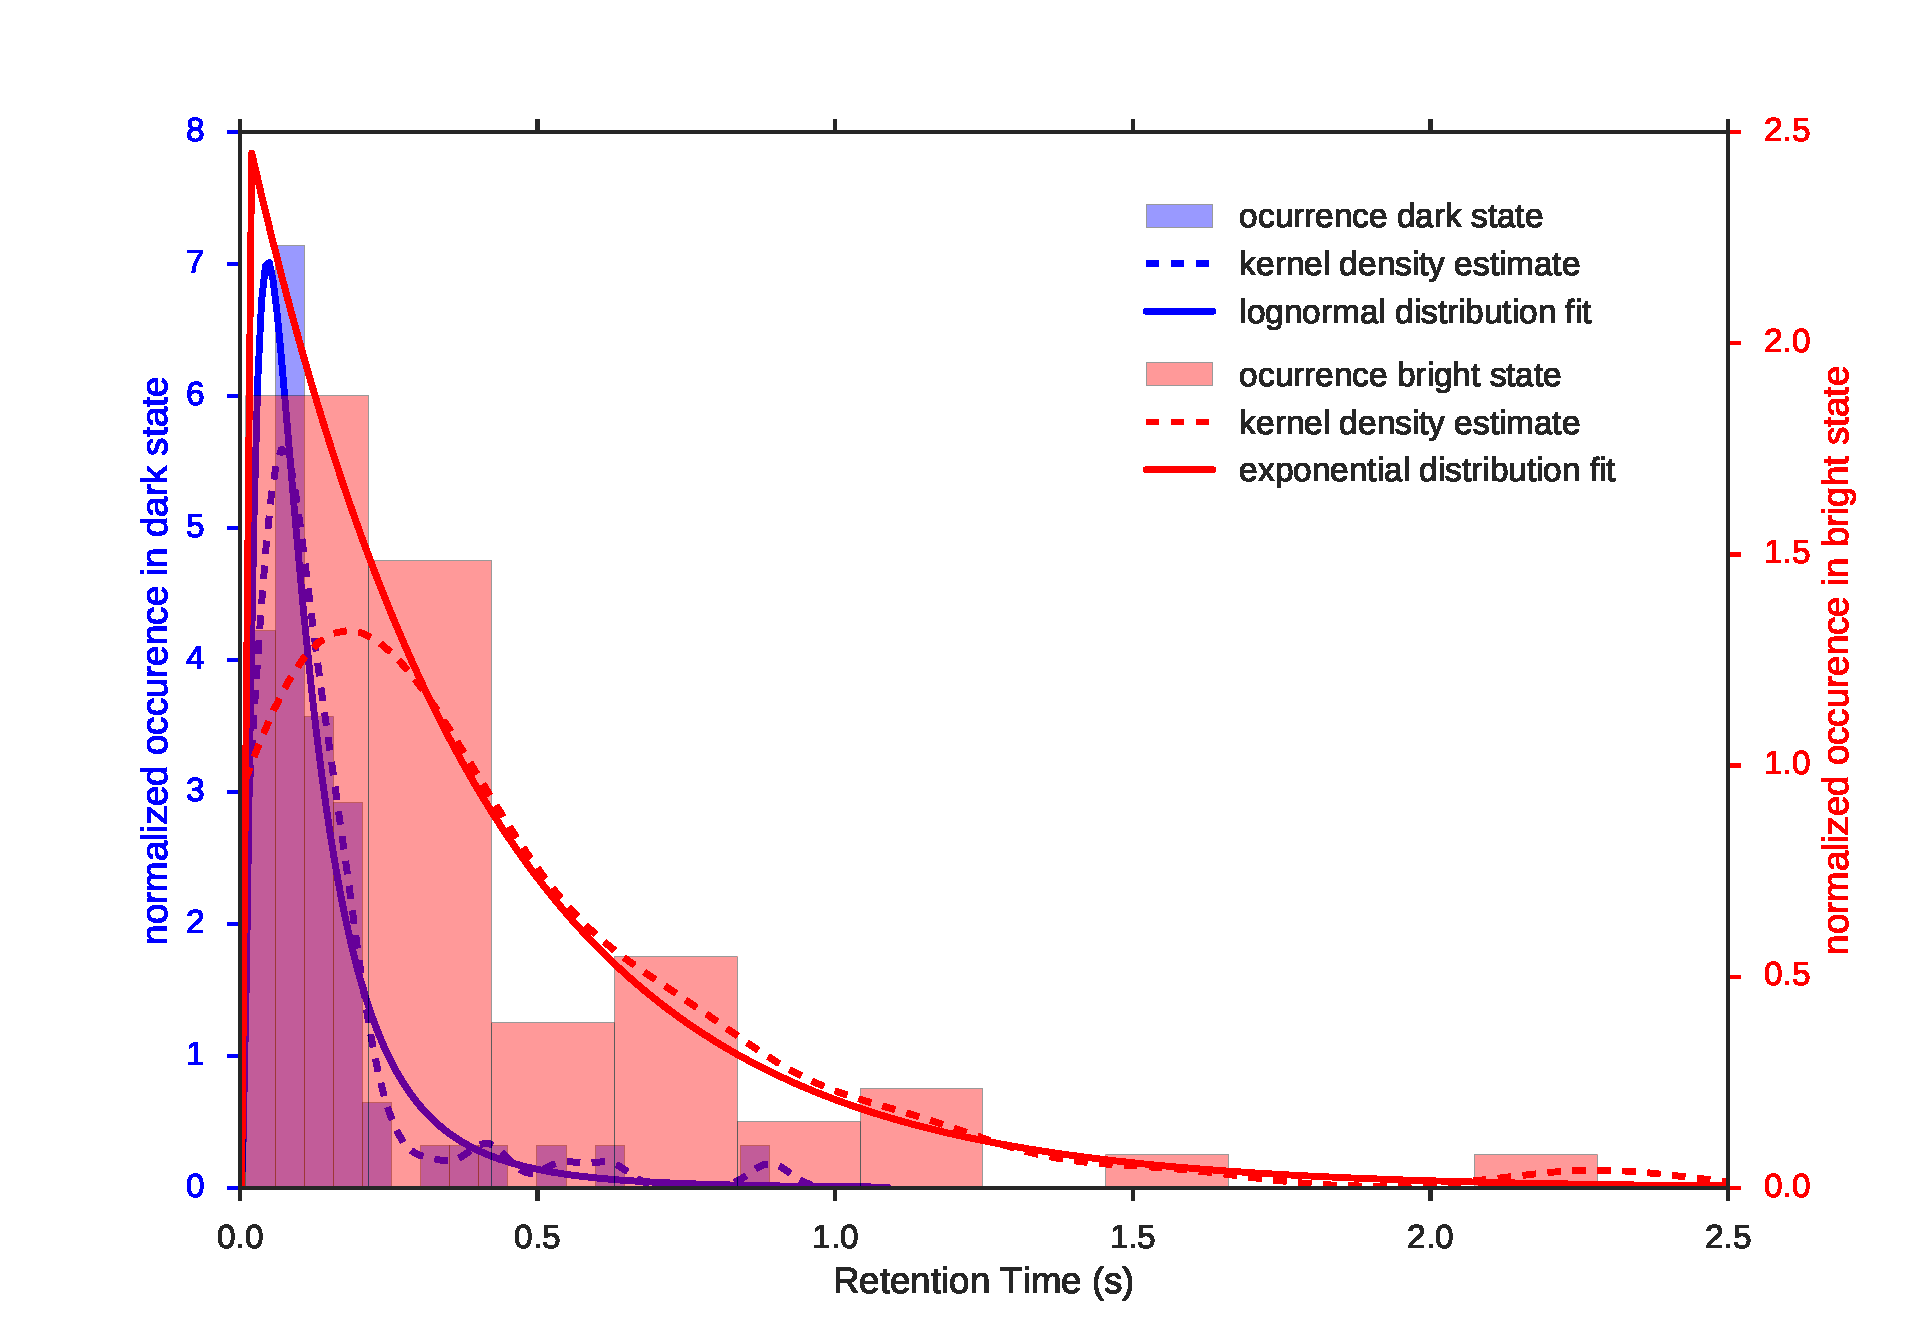
\includegraphics[trim = 0 0 0 0,  clip= true, width = 0.7\textwidth]{./pics/fit_blink_distr_Ir8spe8_xlim2_5.pdf}}
	% 	\caption{Retention times of the single emitter exhibiting the highest blinking rate in the bright (red) and dark (blue) states. The dashed line represents a kernel density estimation of the distribution of retention times. The y-axis is scaled to the normalized kernel density estimate. The red solid line is an exponential fit of the bright state retention times, the blue solid line is a lognormal fit of the dark state retention times. The fits are in good agreement with the data (p-values: red 0.92, blue 0.77)}
	% 	\label{fig::fit_blink_distr}
	% \end{figure}
	%
	% As mentioned in the previous section, the investigated \sivs exhibit count rates of a few thousand to a few \SI{100000}{cps}.
	% To further investigate the count rate, the luminescence time trajectory of the emitters which exhibit a dip at \gtz is evaluated.
	% It is found that some of the observed emitters exhibit fluorescence intermittence, also called blinking (\Fref{fig::blink}).
	% Blinking is attributed to temporal ionization of the color center during optical excitation, forming an optically inactive charge state \cite{Jantzen2016,Neu2012a,Gali2013}.
	% Therefore the emitters change between states of higher and lower emission, i.e. brighter and darker states, called blinking levels.
	% \\
	% The time trace of the emitter is shown in \Fref{fig::blink}.
	% In the overview picture (\Fref{subfig::blink_long}), a few blinking dips can be seen with retention times of up to a few minutes.
	% The fact, that the count rate never drops to the dark count rate lets us assume, that there are at least two \sivs present, one exhibiting fluorescence intermittence and one exhibiting a stable emission.
	% When zooming in, shorter retention times are observable (\Fref{subfig::blink_short}).
	% The retention times range from a few tens of milliseconds up to a few seconds with a few outliers exhibiting very long retention times up to a few hundred seconds.
	% \\
	% The retention times of the bright and of the dark state exhibit different probability distribution functions and with that, different characteristic retention times.
	% The red histogram in \Fref{fig::fit_blink_distr} shows the retention times of the emitter in the bright state, whereas the blue histogram shows the retention times of the dark states (both omitting outliers with very long retention times).
	% The dashed lines are kernel density estimators of the distribution of the respective retention times (i.e. every data point is represented with a Gaussian function and the resulting functions are added up to model the whole data).
	% The red solid line is an exponential fit of the distribution of retention times in the bright state.
	% The high p-value of \num{0.92} confirms the goodness of the fit.
	% The mean and the median retention time in the bright state obtained by the exponential fit amount to \SI[separate-uncertainty]{0.13\pm0.13}{s} and \SI{0.09}{s}, respectively.
	% While other literature about solid state quantum emitters reports an exponential probability distribution for both retention times in bright and dark states \cite{Bradac2010,Berhane2017}, we found a lognormal probability distribution for the retention time in the dark state.
	% The solid blue line in \Fref{fig::fit_blink_distr} is a lognormal fit of the distribution of the retention times in the dark state.
	% With a p-value of \num{0.77} it is by far the best model to describe the data distribution.
	% For comparison: The p-value of an exponential fit only amounts to \num{0.36}.
	% The median retention time in the dark state obtained by the lognormal fit amounts to \SI{0.10}{s}, therefore being a bit longer than the median retention time in the bright state (neglecting very long retention times which are treated as outliers).
	% \\
	% We do not identify a correlation between the count rate of a blinking level and its retention time.
	% However, there is a correlation between the position in the bimodal distribution and blinking:
	% All but one emitters in \hl exhibit blinking, where only one of the emitters in \vl exhibits blinking (\Fref{fig::bimodal_distr}).
	% This dependency suggests that emitters in strained nanodiamonds are more likely to exhibit blinking.
	% \\
	% We explain the observed blinking as a manifestation of the local crystal disorder due to dislocations and impurities which act as a trap for the excited electron and therefore switching the emitter to the dark state \cite{Bradac2010}.
	% The assumption that disloctaions and impurities are responsible for blinking emitters is in agreement with our findings in \ref{subsec::raman}, where we attribute the Raman line at wavenumbers lower than the value of pristine diamond to damage of the diamond lattice.




	\section{Photostability} \label{subsec::photostab}

		\begin{remark}
			Auch hier hab ich einfach mal den gut formulierten text vom paper hineinkopiert. Wenn du aus dem alten text noch sachen einfuegen willst, dann gern. Ich hatte hier den eindruck, dass so ziemlich alles schon da ist, aber vielleicht taeusch ich mich.
		\end{remark}

		As mentioned in the previous section, the single photon count rates observed from the investigated \sivs varies strongly between a few thousand to a few \SI{100000}{cps}.
		To further investigate the count rate, the luminescence time trajectory of the emitters which exhibit a dip at \gtz is evaluated.
		It is found that some of the observed emitters exhibit fluorescence intermittence, also called blinking. \Fref{fig::blink} illustrate the effect.
		Blinking is attributed to temporal ionization of the color center during optical excitation, forming an optically inactive charge state \cite{Jantzen2016,Neu2012a,Gali2013}.
		Therefore the emitters change between states of higher and lower emission, i.e.\ brighter and darker states, called blinking levels.

		\begin{figure}[htp]
			\begin{subfigure}[tp]{ 0.49\linewidth}
				\centering
				\testbox{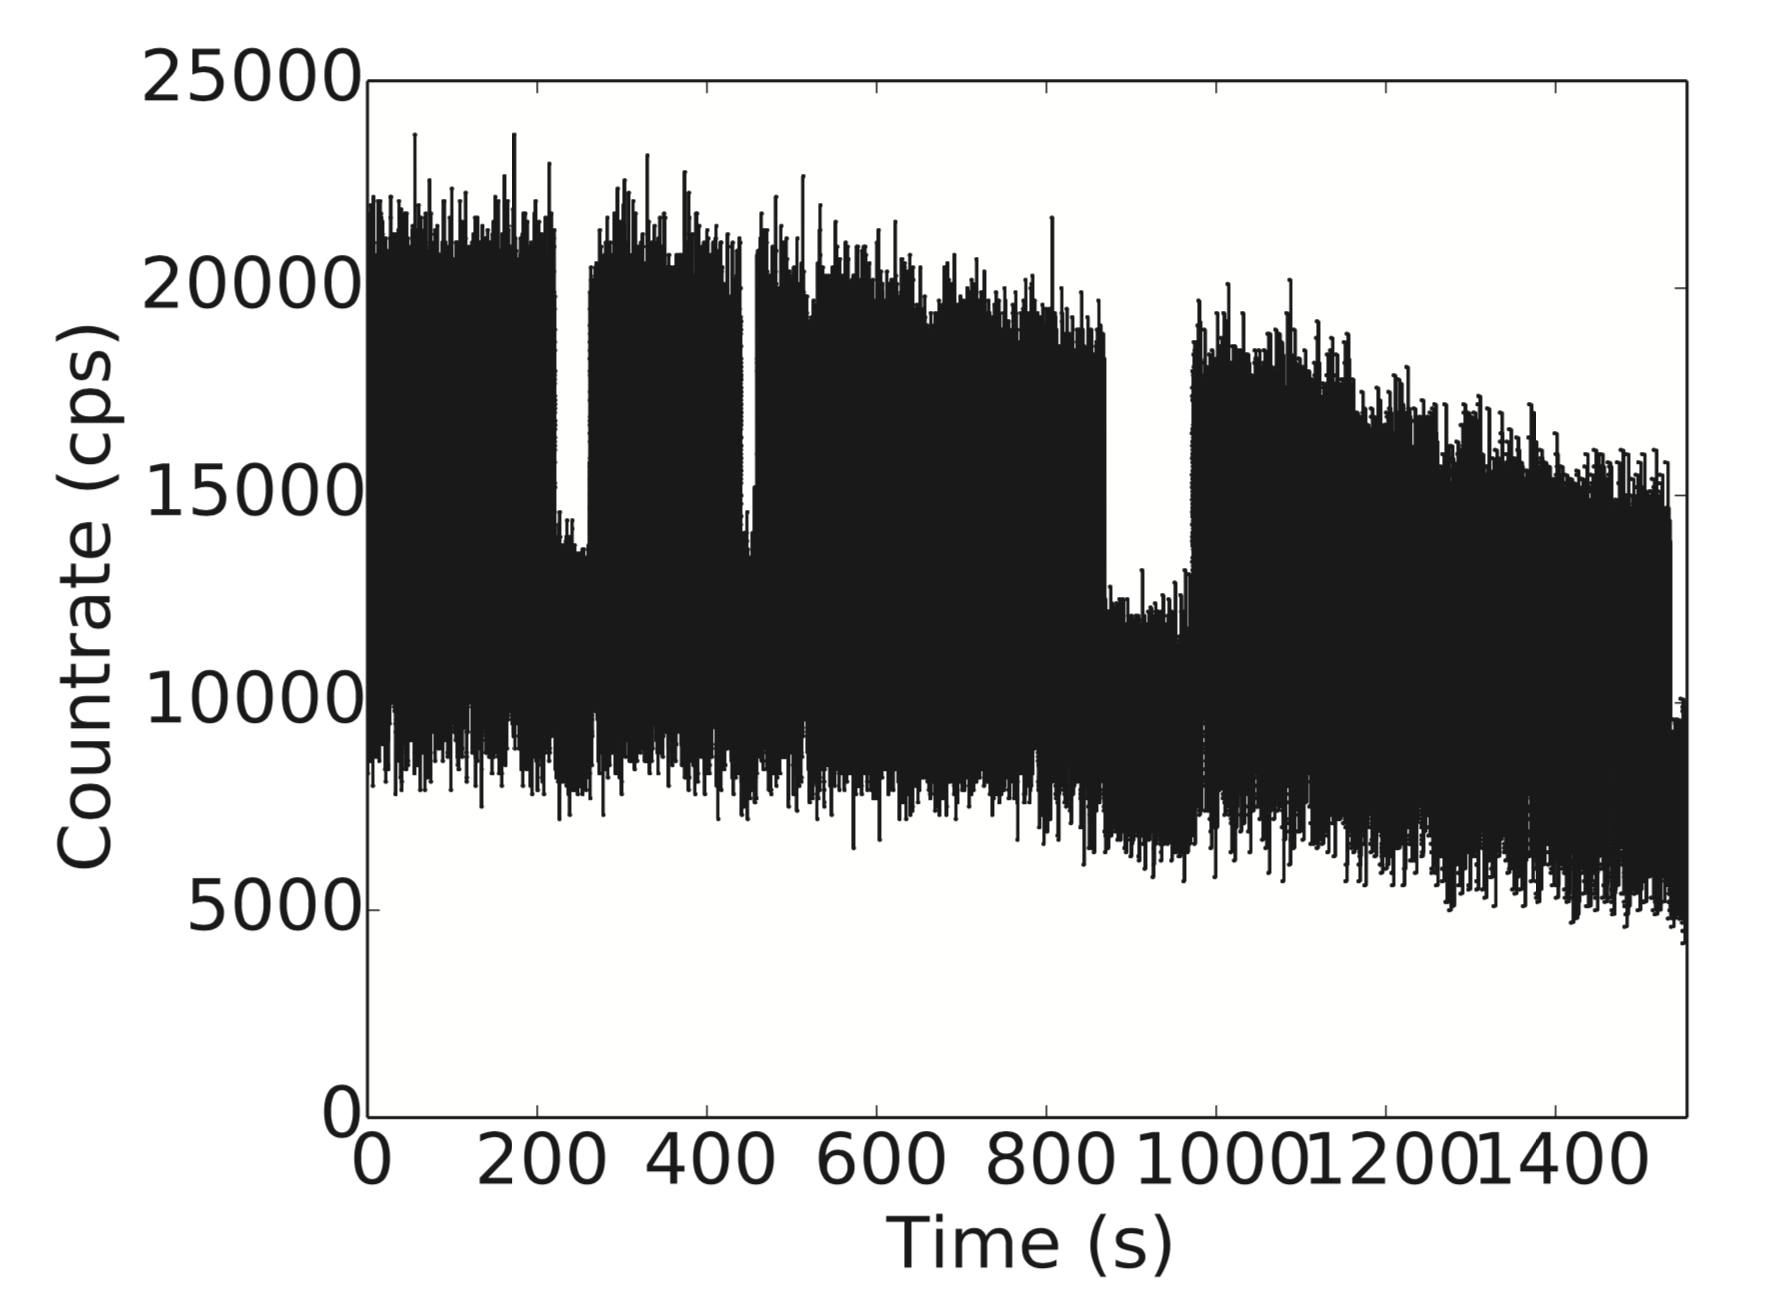
\includegraphics[trim = 0 0 0 0,  clip= true, width = \textwidth]{./pics/g2zuSpektrum8_15_5_countrate_0_01_conv_screenshot.png}}
				\caption{}\label{subfig::blink_long}
			\end{subfigure}
			\hfill
			\begin{subfigure}[tp]{ 0.49\linewidth}
				\centering
				\testbox{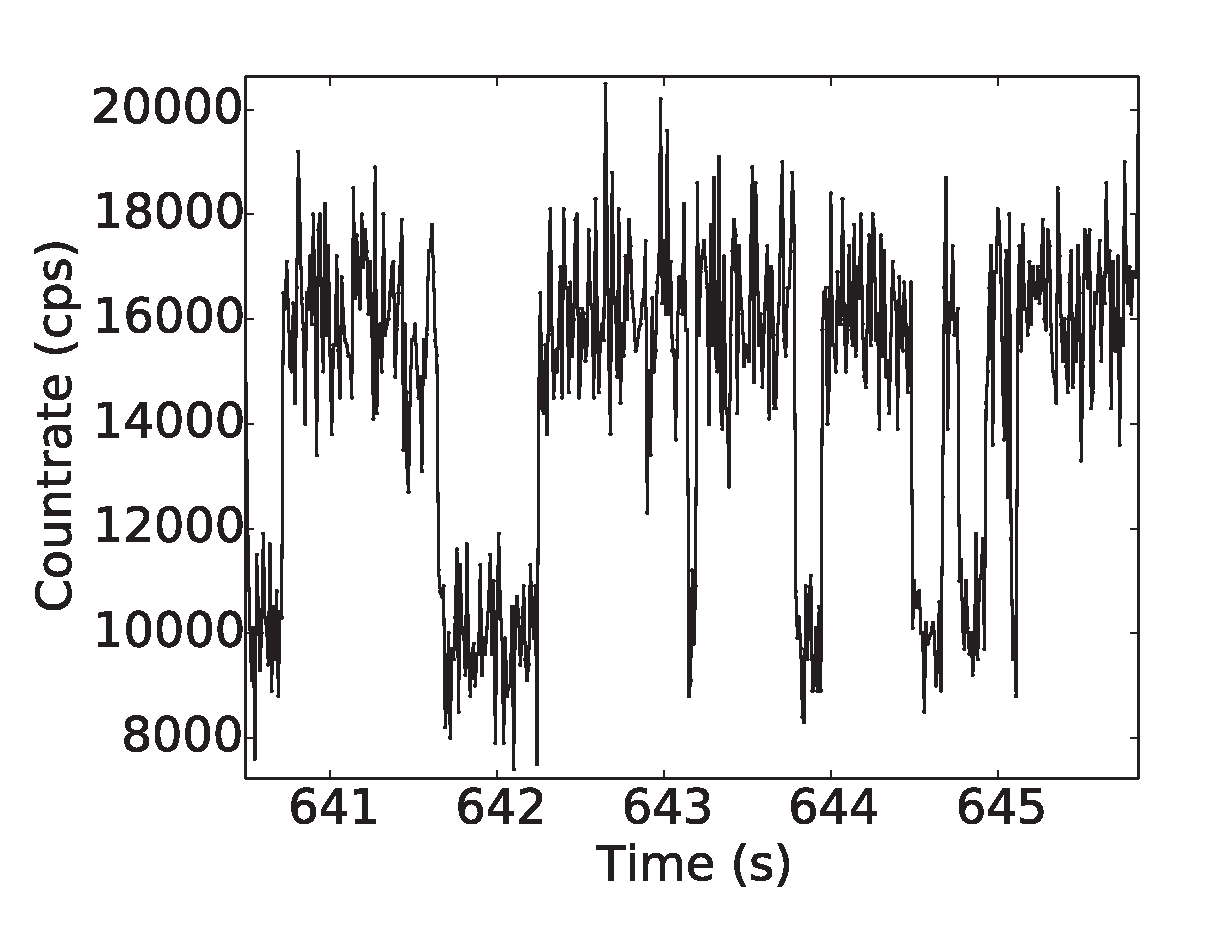
\includegraphics[trim = 0 0 0 0,  clip= true, width =\textwidth]{./pics/g2zuSpektrum8_15_5_countrate_0_01_conv_detail.pdf}}
				\caption{}\label{subfig::blink_short}
			\end{subfigure}
			\caption[Time trace of a single emitter.]{(a) Time trace of the single emitter H1, which exhibits strong blinking. The variation of the count rate in the upper state is attributed to a drift of the setup. (b) Detail of the time trace of the same emitter.}
			\label{fig::blink}
		\end{figure}

		The photon count time trace of emitter \emnarrow is shown in \Fref{fig::blink}.
		In the overview picture (\Fref{subfig::blink_long}), a few blinking dips can be seen with time intervals of up to a few minutes.
		The fact that the count rate never drops down to the dark count rate lets us assume, that there are at least two \sivs present, one exhibiting fluorescence intermittence and one exhibiting a stable emission.
		When zooming in, shorter time intervals are observable (\Fref{subfig::blink_short}).
		The time intervals range from a few tens of milliseconds up to a few seconds with a few outliers exhibiting very long time intervals up to a few hundred seconds.
		\\
		The bright and dark times exhibit different probability distribution functions and with that, different characteristic time constants.
		In \Fref{fig::fit_blink_distr} the time intervals of the emitter are shown as small vertical dashed red lines and solid blue lines for the bright and dark state respectively.

		\begin{figure}[htp]
			\centering
			\testbox{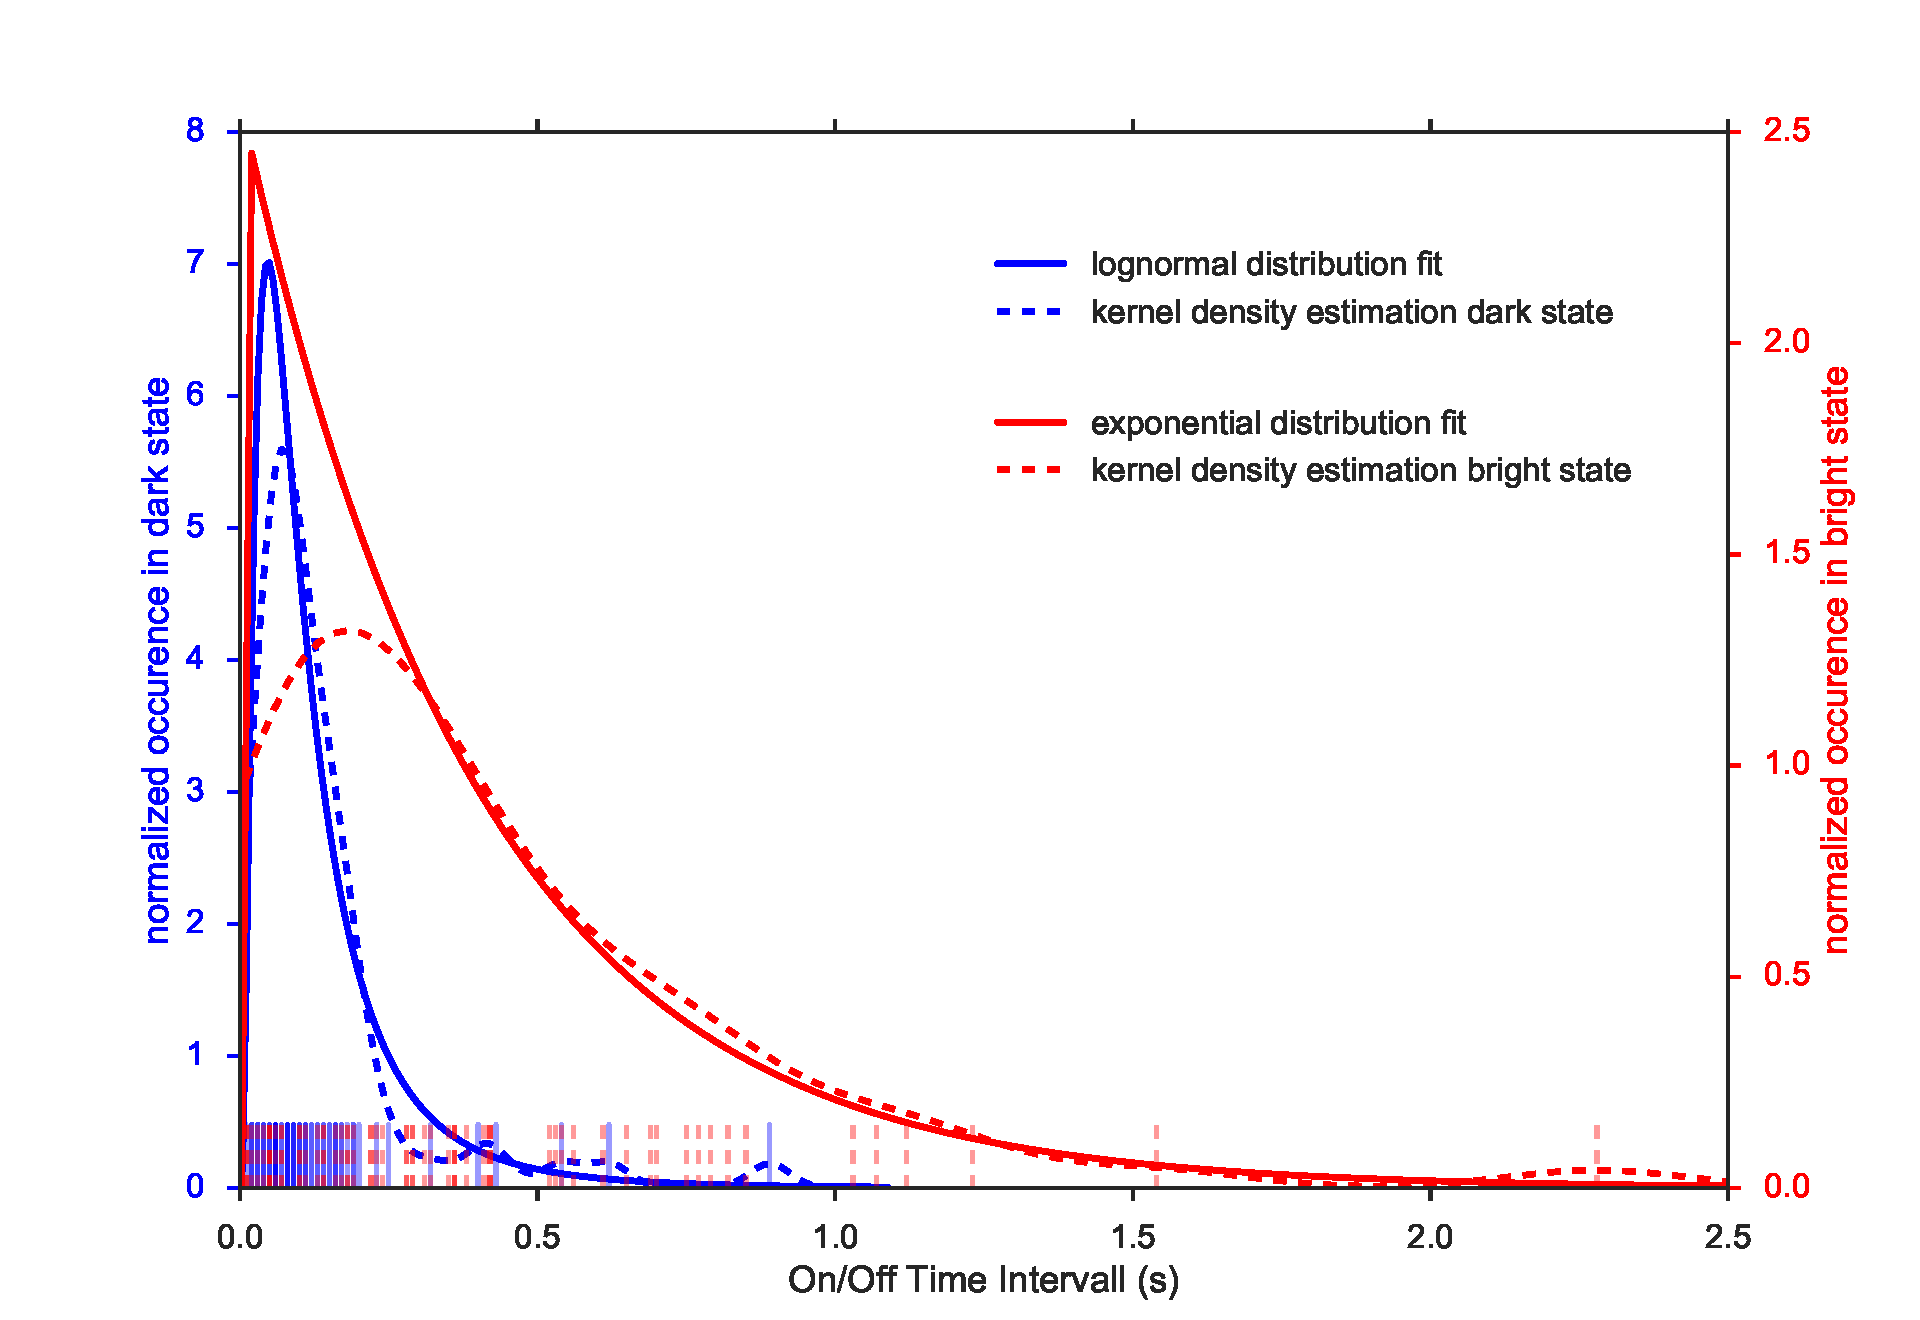
\includegraphics[trim = 0 0 0 0,  clip= true, width = 0.7\textwidth]{./pics/retention_no_histo_xlim2_5.pdf}}
			\caption[Distributions of brigth and dark state intervals]{Time intervals of the single emitter exhibiting the highest blinking rate in the bright (red) and dark (blue) states. Each flank of the blinking state was individually read out from the \pl time trace. On the horizontal axis small vertical lines represent the individual data points of the bright/dark time intervals. The blue and red dashed curves represent kernel density estimations of the distribution of time intervals of the dark and bright states, respectively. The y-axis is scaled to the normalized kernel density estimate. The red solid line is an exponential fit of the bright state time intervals whereas the blue solid line is a log-normal fit of the dark state time intervals. These fitting functions were chosen because they provide the best agreement with the data using a Kolomogorov-Smirnov test with respect to other functions (p-values: bright state (red) 0.92, dark state (blue) 0.77).}
			\label{fig::fit_blink_distr}
		\end{figure}

		Outliers with very long time intervals are ommited here.
		The dashed lines are kernel density estimators of the distribution of the respective time intervals.
		This implies that every data point is represented with a Gaussian function and the resulting functions are added up to model the whole data.
		The red solid line is an exponential fit of the distribution of time intervals in the bright state.
		The high p-value of \num{0.92} confirms the goodness of the fit.
		The median time interval in the bright state obtained by the exponential fit amounts to \SI[separate-uncertainty]{0.09}{s}.
		While other literature about solid state quantum emitters reports an exponential probability distribution for both time intervals in bright and dark states\cite{Bradac2010,Berhane2017}, we found a log-normal probability distribution for the time interval in the dark state.
		The solid blue line in \Fref{fig::fit_blink_distr} is a log-normal fit of the distribution of the time intervals in the dark state.
		A Kolomogorov-Smirnov test yields a p-value of \num{0.77} for the log-normal fit and is by far the best model to describe the data distribution.
		For comparison: The p-value of an exponential fit amounts to \num{0.36}.
		The median time interval in the dark state obtained by the log-normal fit is determined as \SI{0.10}{s}, therefore being close to the median time interval in the bright state.
		Very long time intervals are not shown in the plot for better visualization of the small timescales, however these long time intervals are included in the fit.
		The longest measured time interval amounted to \SI{41.14}{s} and occurred in the dark state.
		\\
		Measurements of blinking time intervals in \cite{Jantzen2016} and \cite{Neu2012a} report time intervals between about \SIrange{0.03}{1}{s}, and \SI{0.1}{s} to \SI{2}{min}, respectively.
		These findings are in good agreement with our measurements.
		\\
		In general, excitation and emission process is mediated by charge separation (i.e.\ excitons).
		If an electron or hole is localized far enough that there is sufficiently negligible overlap with the wave function of the remaining carrier, blinking occurs \cite{Efros2016}.
		We explain the observed blinking as a manifestation of the local crystal disorder due to dislocations and impurities which act as a trap for the excited electron and therefore switch the emitter to the dark state.
		The capture of the electron of the exciton by traps due to local crystal disorders may inhibit recombination and therefore induce the dark state \cite{Bradac2010}.
		The assumption that dislocations and impurities are responsible for blinking emitters is in agreement with our findings reported in \ref{subsec::raman}.
		\\
		Research of blinking rhodamine molecules confirms power law distributed bright state times and log-normal distributed dark state times \cite{Wong2013}.
		The log-normal distribution is explained by a Gaussian distribution of activation barriers of the electron transfer to trap states in the surrounding material \cite{Albery1985}.
		It hints towards a recapture of the electron via multiphonon relaxation channels.
